\documentclass[a4paper]{report}

\usepackage{graphicx}
\usepackage[english]{babel}
\usepackage[utf8]{inputenc}
\usepackage[T1]{fontenc}
\usepackage{ragged2e}
\usepackage{hyphenat}
\usepackage{lmodern}
\usepackage{fancyhdr}
\usepackage[toc,page]{appendix}
\usepackage{tabularx}
\usepackage{float}
\usepackage{amsmath}
\usepackage{indentfirst}

\setcounter{secnumdepth}{4}

\begin{document}
    \centering
    \LARGE{\textsc{VIETNAM AVIATION ACADEMY}}\\
    \vspace{3mm}
    \normalsize{Department of Telecommunication - Electronics Engineering Technology} \\
    \vspace{3mm}
    \large{LOCATION IN HO CHI MINH CITY} \\
    \vspace{3mm}
    
\includegraphics[scale=0.3]{logo.jpg} \\
    \vspace{3mm}
    \normalsize{PROJECT REPORT: } \\ 
    \vspace{15mm}
    \huge{\textbf{"Radar detector module using Arduino"}} \\
    \vspace{20mm}
    \normalsize{Written by} \\
    \vspace{3mm}
    \large{\textbf{\textit{Nguyen Van Anh Tuan}}} \\
    \vspace{3mm}
    \textbf{{\large{\textit{Roll.No.1753020018}}}} \\
    \vspace{15mm}
    \large{Under the guidance of} \\ 
    \vspace{10mm}
    \centerline{\textbf{\large{Cao Xuan Kim Anh}}}
    
    %Lines down here is set header and footer
    \pagestyle{fancy}
    \fancyhf{}
    \rhead{Radar detector module}
    \lhead{Anh Tuan}
    \cfoot{\today}
    \renewcommand{\headrulewidth}{2pt}
    \renewcommand{\footrulewidth}{1pt}

    % \setlength\parindent{24pt} is indentation.
    \newpage
    \centering
    \centerline{\textbf{\huge{PREAMBLE}}}
    \vspace{10mm}
    \begin{flushleft}
        Radar is an object detection system. It uses Microwaves to determine the range, 
        altitude, or speed of objects. The radar can transmit radio waves or microwaves 
        which bounce off any object in their path. So, we can easily determine any object 
        in the radar range. Arduino is a single-board microcontroller to make electronics 
        more discipline. The radar system has different performance specifications and also 
        it comes in a verity of size.
    \end{flushleft}
    \begin{flushright}
        \textbf{Auth. Nguyen Van Anh Tuan}
    \end{flushright}
    \thispagestyle{plain}

    \newpage
    \tableofcontents

    \chapter{Introduction}
    \thispagestyle{fancy}
    \fancyhf{}
    \fancyhead[L]{Anh Tuan}
    \fancyhead[R]{Radar detector module}
    \raggedright
    \fancyfoot[R]{Page \thepage}
    \section{PRELIMINARY INTRODUCTION}
    \subsection{The reason why to choose project}
        With the passion for aviation as well as passion for technology and equipment realted to 
        it, i decided to choose an aviation-related project in this project. Fortunately, my project 
        this time is on topic of embedded programming. So, i choose project named "NDB radar 
        detector module using Arduino". In this project, i will rely 
        on the NDB radar to make a small scale NDB radar detector model. So, to get 
        started in this project, we need to know what NDB radar is and how it works. \\
    \vspace{5mm}
        Recognize the continuous development of aviation technology. I want to add my own 
        knowledge about how a radar system works and a bit of creative idea for this device 
        that came along during i make this project. And that's why i choose this project for myself. \\
    \vspace{5mm}
    \textbf{Block diagram}
    \begin{figure}[ht]
        \centering
        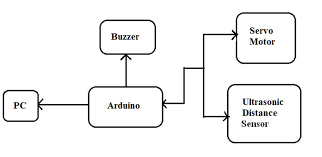
\includegraphics[scale=0.7]{block_diagram.png}
        \caption{\label{fig:pic}Block diagram for radar model}
    \end{figure}
    \linebreak
    \par You may ask how the processing application works here. It's very simple, the 
    Ultrasonic sensor collects the object information with the help of Arduino and passes 
    it to processing application, there is a simple Graphics application implemented which 
    mimic a radar screen.
    \subsection{Target Research}
        The short term goal of this topic is with the desire to learn and supplement the 
        knowledge that in the course of research. With the long term goal, i want to perform 
        the topic in the best way i can. As well as improve the errors of myselft. And also, 
        i want to additional the knowledge i haven't learned at my school.
    \subsection{Object and position research}
    \vspace{3mm}
        \begin{itemize}
            \item \textbf{Object Research:} The object that i study is the sensor system 
        installed on the air traffic control station or installed on robots that detect 
        objects and avoid them.
            \item \textbf{Position Research:} My reserach is based on the application of radar 
        to detect missing vehicles or to apply air traffic control as call as "Primary Surveillance Radar".
        \end{itemize} 
    \subsection{Method of research}
        \begin{itemize}
            \item \textbf{Observation Method:} By observing directly at air traffic control 
        and also via movies or aviation videos on internet.
            \item \textbf{Method of analysis:} Looking for some similar projects that have 
        been made available online, from the detailed data of those projects, i draw some 
        methods and experience for my project. Avoid mistakes in my project.
        \end{itemize}
    \subsection{Structure Project}
        My article is divided into three main sessions, summarized as follow: 
        \begin{itemize}
            \item In the first chapter, i will focus on brief introduce my project, presenting 
        some of the research content on the topic of the method of conducting research that 
        gives practical results during the project research process.
            \item The second chapter, is an introduction about some of basic project implementation 
        theories, to present related project i'm working on it.
            \item Chapter three is the chapter where i introduce the main content of my project, 
        presenting a basic article of project and how it works, accompany it with some examples.
            \item The next chapter is the construction and circuit design on Kicad Altium software 
        and the implementation of hardware construction.
            \item And the final chapter is the final section where i draw some conclusion during 
        project implementation, as well as point out my own strengths weaknesses in the course of my project.
        \end{itemize}
    \newpage
    \section{BASIC THEORY}
    \subsection{Some research related to the project}
        Some research ideas related to my project:
        \begin{itemize}
            \item The function contained in some robots, helps robots scan the terrain 
        and detect objects to avoid.
            \item Radar in the Air traffic control tower named "Primary Surveillance Radar"
        \end{itemize}
    \subsection{Theory concepts related to research issues}
        \begin{itemize}
            \item \textbf{PSR(Primary Surveillance Radar)}: A Surveillance radar system which
        uses reflected radio signals.
            \item \textbf{US(Ultrasonic Sensor)}: As the name indicates, ultrasonic sensors 
        measure distance by using ultrasonic waves.
            \item \textbf{PWM(Pulse-Width Modulation)}: is a method of reducing the average 
        power delivered by an electrical signal, by effectively chopping it up into discrete parts.
            \item \textbf{RAM(Random-Access Memory)}: is a form of computer memory that can be 
        read and changed in any order, typically used to store working data and machine code.
            \item \textbf{CPU(Central Processing Unit)}: also called a central processor or main 
        processor, is the electronic circuitry within a computer that executes instruction that 
        make up a computer program.
        \end{itemize}
    \subsection{Components Required}
        \begin{enumerate}
            \item For power:
            \setlength{\parindent}{4em}
            Micro USB-B
            \item For radar model:
            \begin{enumerate}
                \item Arduino UNO
                \item Servo motor
                \item Ultrasonic Sensor HRF-04
                \item Buzzer
                \item LCD 16x02
                \item LED (green, red)
                \item Test board
            \end{enumerate}
        \end{enumerate}
    \newpage
    \subsection{Component Description}
        \vspace{3mm}
        \subsubsection{\Large{Arduino Uno}}
            \vspace{3mm}
            \begin{enumerate}
                \item \textbf{Introduction about Arduino UNO}
                \linebreak
                \par Arduino UNO is a microcontroller board developed by Arduino.cc which is open-source 
                electronics platform mainly based on AVR microcontroller ATMega328. \\
                \vspace{3mm}
                \par First Arduino projcet was started in Interaction Design Institute 
                Ivrea in 2003 by David Cuartielles and Massimo Banzi with the intention of 
                providing a cheap and flexible way to students and professional for controlling 
                a number of devices in the real world. \\
                \vspace{3mm}
                \par The current version of Arduino UNO comes with USB interface, 6 analog 
                input pins, 14 I/O(input/output) digital ports that are used to connect with 
                external electronic circuit. Out of 14 I/O ports, 6 pins can be used for PWM output.\\
                \vspace{3mm}
                \par It allows the designers to control and sense the external electronic devices in 
                the real world. \\
                \vspace{3mm}
                \par Apart from USB, battery or AC to DC adopter can also be used to power the board. \\
                \vspace{3mm}
                \par There are many versions of Uno board available. However, Arduino Uno V3 and Arduino 
                Uno are the most official versions that come with ATMega328 8-bit AVR Atmel microcontroller 
                where RAM memory is 32KB.
                \begin{figure}[ht]
                    \centering
                    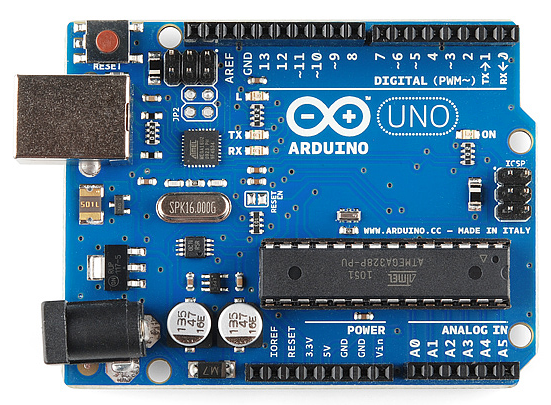
\includegraphics[width=0.5\linewidth]{Uno.png}
                    \caption{\label{fig:pic}Arduino Uno board}
                \end{figure}
                \item \textbf{Features}
                    \linebreak
                    \begin{figure}[ht]
                        \centering
                        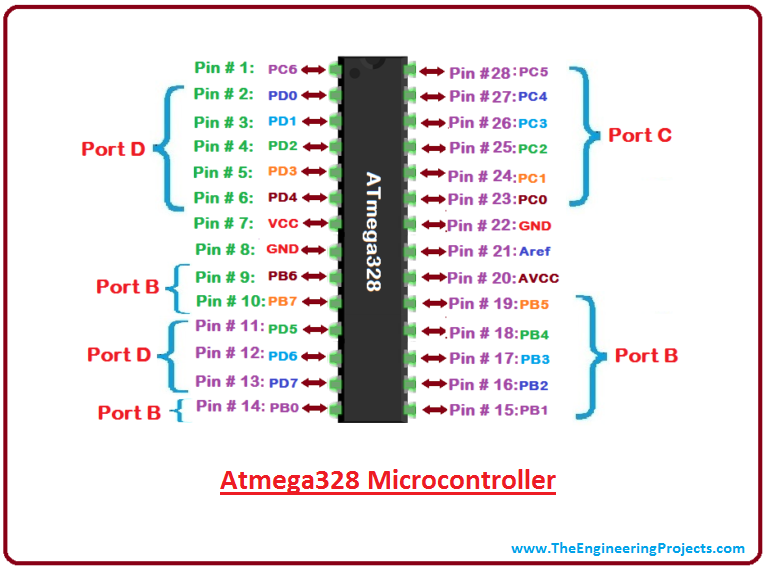
\includegraphics[width=0.6\linewidth]{atmega.png}
                        \caption{\label{fig:pic}ATMega328 Microcontroller}
                    \end{figure}
                \begin{itemize}
                    \item Comes with USB interface.
                    \item USB port is added on the board to develop serial communication with the computer
                    \item ATMega328 microcontroller is placed on the board that comes with a number of 
                features like timers, counters, interrupts, PWM, CPU, I/O pins and based on a 16MHz clock 
                that helps in producing more frequency and number of instruction per cycle.
                    \item It's an open-source platform where anyone can modify and optimize the 
                board based on the number of instructions and task they want to achieve.
                    \item Come with a built-in regulation feature which keeps the voltage under control 
                when the device is connected to the external device.
                    \item There are 14 pins I/O digital and 6 analog pins in the board that allows the 
                external connection with any circuit with the board. These pins provide the flexibility 
                and ease of use to the external devices that can be connected through these pins.
                    \item 6 analog pins are marked as A0 to A5 and come with a resolution of 10bits. 
                These pins measure from 0V to 5V, however, they can be configured to the high range 
                using analogReference() function and AREF pin.
                    \item 13KB of flash memory is used to store the number of instructions in the form 
                of code.
                    \item Only 5V is required to turn the board on, which can be achieved directly using 
                USB port or external adopter, however, it can support external power source up to 12V 
                which can be regulated and limit to 5V or 3.3V based on the requirement of the project. 
                \end{itemize}
                \item \textbf{Pinout}
                    \linebreak
                    \vspace{3mm}
                    \par Arduino Uno is based on AVR microcontroller call ATMega328. This controller 
                comes with 2KB RAM, 32KB of flash memory, 1KB of EEPROM. Arduino board comes with 
                14 digital pins and 6 analog pins.
                    \begin{figure}[ht]
                        \centering
                        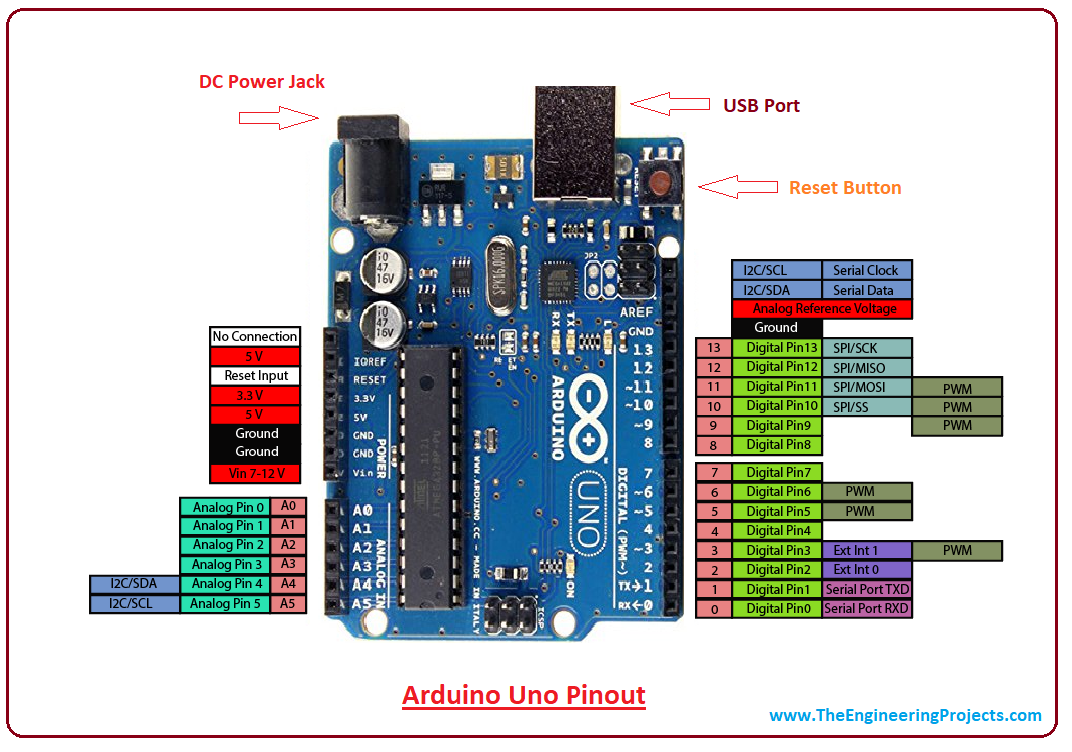
\includegraphics[width=\linewidth]{pinout.png}
                        \caption{\label{fig:pic}Arduino Uno Pinout}
                    \end{figure}
                \item \textbf{Pin Description}
                    \linebreak
                    \vspace{3mm}
                    \par \textbf{LED:} comes with build-in LED which is connected through pin 13.
                Providing HIGH value to the pin will turn it ON and LOW will turn it OFF. \\
                    \vspace{2mm}
                    \par \textbf{Vin:} input voltage provided to the Arduino Uno board. It's
                different than 5V supplied through the USB port. This pin is used to supply voltage. 
                If a voltage is provided through power jack, it can be accessed through this pin. \\
                    \vspace{2mm} 
                    \par \textbf{5V:} comes with the ability to provide voltage regulation. 5V pin is 
                used to provide output regulated voltage. The board is powered up using the 3 ways: 
                USB, Vin pin of the board or DC power jack. \\
                    \vspace{2mm}
                    \par \textbf{GND:} ground pins. More than one ground pins are provided 
                on the board which can be used as per requirement.
                    \vspace{2mm}
                    \par \textbf{Reset:} this is incorporated on the board which resets the 
                program running on the board. Instead of physical reset on the board, IDE comes 
                with a feature of resetting the board through programming. \\
                    \vspace{2mm}
                    \par \textbf{IOREF:} this pin very useful for providing voltage reference to 
                the board. A shield is used to read the voltage across this pin which then select 
                the proper power source. \\
                    \vspace{2mm}
                    \par \textbf{PWM:} is provided by 3,5,6,9,10; 11 pins. These pins are configured 
                to provided 8-bit output PWM. \\
                    \vspace{2mm}
                    \par \textbf{SPI:} It is known as Serial Peripheral Interface. 4 pins 10(SS), 11(MOSI), 
                12(MISO), 13(SCK) provide SPI coummunication with the help of SPI library. \\
                    \vspace{2mm}
                    \par \textbf{AREF:} called Analog Reference. This pin is used for providing a reference 
                voltage to the analog inputs. \\ 
                    \vspace{2mm}
                    \par \textbf{TWI:} called Two-tire Interface. TWI communication is accessed through 
                Wire Library. A4 and A5 pins are used for this purpose. \\
                    \vspace{2mm}
                    \par \textbf{Serial Communication:} is carried out through 2 pins call pin 0(Rx) and 
                pin 1(Tx). Rx pin is used to receive data while Tx pin is used to transmit data. \\
                    \vspace{2mm}
                    \par \textbf{External Interrupts:} Pin 2 and 3 are used for providing external interrupts. 
                An interrupt is called by providing LOW or changing value.
                \item \textbf{Communication and Programming} 
                    \linebreak
                    \vspace{3mm}
                    \par Arduino Uno comes with an ability of interfacing with other Arduino boards, 
                microcontrollers and computer. The ATMega328 placed on board provides serial communication 
                using pins like Rx and Tx. \\ 
                    \vspace{2mm}
                    \par Arduino Uno is programmed using Arduino Software which is a cross-platform application 
                call IDE(Intergrated Development Environment) written in Java. The AVR microcontroller ATMega328 
                laid out on the base comes with built-in bootloader that sets you free from using a separate 
                burner to upload the program on the board.
                \item \textbf{Application}
                    \linebreak
                    \vspace{3mm}
                    \par Arduino Uno comes with a wide range of Applications. A larger number of people 
                are using Arduino boards for developing sensors and instruments that are used in scientific 
                research. Following are some main applications of the board: \\
                    \vspace{2mm}
                    \par \guillemotright Embedded System \\
                    \par \guillemotright Security and Defense System \\
                    \par \guillemotright Digital Electronics and Robotics \\
                    \par \guillemotright Parking Lot Counter \\
                    \par \guillemotright Weighing Machines \\
                    \par \guillemotright Traffic Light Count Down Timer \\
                    \par \guillemotright Medical Instrument \\
                    \par \guillemotright Emergency Light for Railways \\
                    \par \guillemotright Home Automation \\ 
                    \par \guillemotright Industrial Automation \\
                    \vspace{2mm}
                    \par There are a lot of other microcontrollers available in the market that are 
                more powerful and cheap as compared to Arduino board. \\
                    \vspace{2mm}
                    \par Actually, Arduino comes with a big community that is developing and sharing the 
                knowledge with a wide range of audience. Quick support is available pertaining to technical 
                aspects of any electronic project.
            \end{enumerate}
        \subsubsection{\Large{Servo Motor}}
            \begin{enumerate}
                \item \textbf{Introduction}
                    \vspace{3mm}
                    \par Servo Motors(or servos) are self-contained electric devices that rotate or push 
                parts of machine with great precision. Servos are found in many places, from toys to home 
                electronics to cars and airplanes. If you have a radio-controlled model car, airplanes, 
                or helicopter, you are using at least a few servos. By rotating a shaft connected to the 
                engine throttle, a servo regulates the speed of a fuel-powered car or aircraft. \\
                    \vspace{2mm}
                    \par Servo also appear behind the scene in devices we use every day. Electronic device 
                such as DVD players use servos to extend or retract the disc trays.
                    \begin{figure}[ht]
                        \centering
                        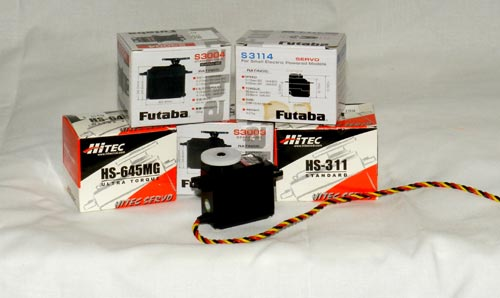
\includegraphics[width=0.6\linewidth]{Servo.jpg}
                        \caption{\label{fig:pic}Assortment of Servos}
                    \end{figure}
                \item \textbf{How does a servo work?}
                    \vspace{3mm}
                    \par The simple of a servo among the features that make them so reliable. 
                The heart of a servo is a small direct current (DC) motor, similar to what you 
                might find in an cheap toy. These motors run on electricity from a battery and spin 
                at high RPM(Rotations per minute) but put out very low \textbf{torque}(a twisting force 
                used to do work you apply torque when you open a bottle).
                    \begin{figure}[ht]
                        \centering
                        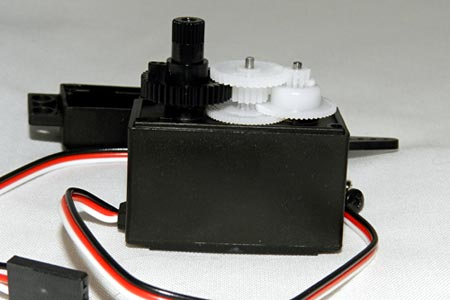
\includegraphics[width=0.6\linewidth]{Servo1.jpg}
                        \caption{\label{fig:pic}The Gears in a Typical Standard-size servo}
                    \end{figure}
                    \newpage
                    \par In high-power servo, the plastic gears are replaced by metal ones for strength. 
                    The motor is usually more powerful than in a low-power servo and the overall output torque 
                    can be as much as 20 times higher than a cheaper plastic one. Better quality is more 
                    expensive, and high-output servos can cost two or three times as much as standard ones.
                    \begin{figure}[ht]
                        \centering
                        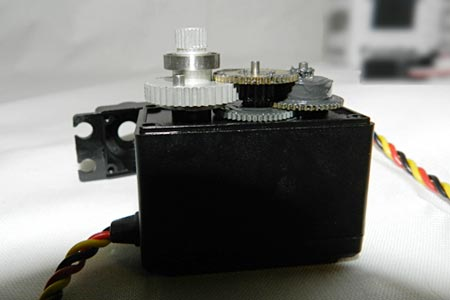
\includegraphics[width=0.6\linewidth]{Servo2.jpg}
                        \caption{\label{fig:pic}The gears in a Typical High-power servo}
                    \end{figure} 
                    \vspace{2mm}
                    \par With a small DC motor, you apply power from a battery, and the motor spins. 
                Unlike a simple DC motor, however, a servo's spinning motor shaft is slowed way down with 
                gears. A positional sensor on the final gear is connected to a small circuit board. The 
                sensor tells this circuit board how far the servo output shaft has rotated. The electronic 
                input signal from the computer or the radio in a remote-controlled vehicle also feeds into 
                that circuit board. The electronics on the circuit board decode the signals to determine 
                how far the user wants the servo to rotate. Then compares the desired position to the 
                actual position and decides which direction to rotate the shaft so it gets to the desired 
                position.
                    \begin{figure}[ht]
                        \centering
                        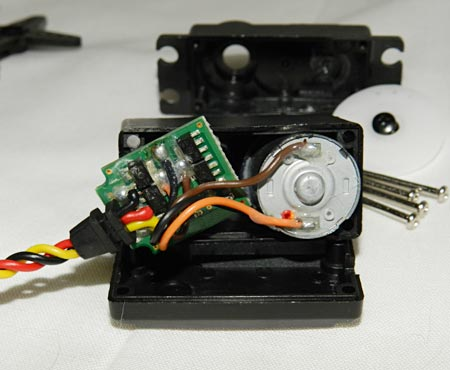
\includegraphics[width=0.4\linewidth]{Servo3.jpg}
                        \caption{\label{fig:pic}The circuit board and DC motor in a high-power servo}
                    \end{figure}
                \item \textbf{Types of servo motors}
                    \vspace{3mm}
                    \par Servos come in many sizes and in 3 basic types: 
                    \begin{itemize}
                        \item \textbf{Positional rotation servo:} This is the most common type of servo 
                    motor. The output shaft rotates in about half of a circle, or 180 degrees. It has physical 
                    stops placed in the gear machanism to prevent turning beyond these limits to protect the 
                    rotational sensor. These common servos are found in radio-controlled cars, aircraft, toys, 
                    robots and many applications. 
                        \item \textbf{Continuous rotation servo:} This is quite similar to the common positional 
                    rotation servo motor, except it can turn in either direction indefinitely. The control 
                    signal, rather than setting the static position of the servo, is interpreted as the direction 
                    and speed of rotation. The range of possible commands causes the servo to rotate clockwise 
                    or counterclockwise as desired, at varying speed, depending on the command signal. You might 
                    use a servo of this type on a radar dish if you mounted one on a robot. Or you could use 
                    one as a drive motor on a mobile robot.
                        \item \textbf{Linear servo:} This is also like the positional rotation servo motor described 
                    above, but with additional gears(usually a \textbf{rack and pinion} mechanism) to change 
                    the output from circular to back-and-forth. These servos are not easy to find, but you can 
                    sometimes find them at hobby stores where they are used as actuators in larger model airplanes.
                    \end{itemize}
                \item \textbf{Selecting a servo motor}
                    \linebreak
                    \vspace{3mm}
                    \begin{figure}[ht]
                        \centering
                        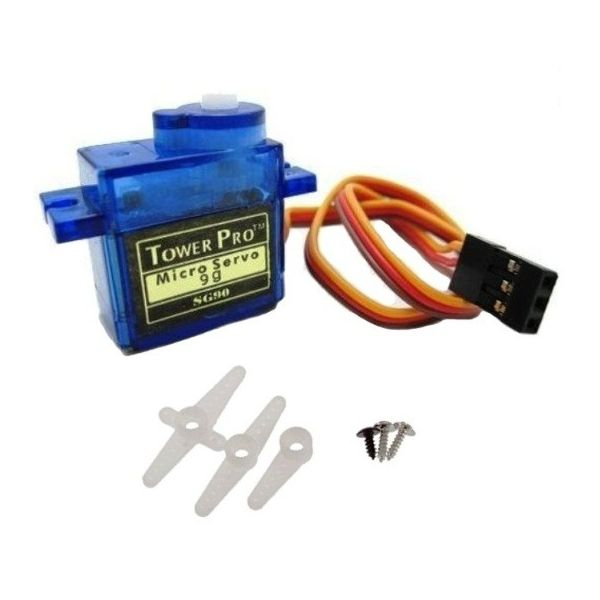
\includegraphics[width=0.3\linewidth]{sg90.jpg}
                        \caption{\label{fig:pic}Micro Servo 90}
                    \end{figure}
                    \newpage
                    Micro servo motor 90(SG90) is tiny and lightweight with high output power. This servo can 
                    rotate approximately 180 degrees (90 in each direction), it works just like the standard kinds 
                    but smaller. We can use any servo code, hardware or library to control this servo.
            \end{enumerate}
\end{document}